% Soporte local de firma para el cuerpo y los anexos del Subdocumento 8.
% No altera la clase ni las plantillas compartidas.
\newcommand{\LFXportadasd}{%
  \AddToHookNext{shipout/foreground}{%
    \begin{tikzpicture}[remember picture,overlay]
      \node[anchor=north west,inner sep=0pt]
        at \LFXen{\LFXmi}{0.835}
        {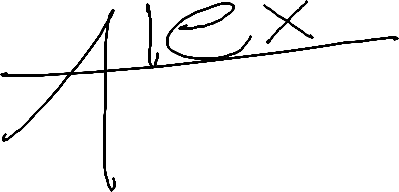
\includegraphics[height=13mm]{logo/FIRMA_Alex_Aravena_transparente.png}};
    \end{tikzpicture}%
  }%
  \portadalafrox
}

% Firma abreviada sobre filete, en el mismo espacio del pie existente.
\renewcommand{\LFXpiederecho}{%
  \begingroup\LFXpiebase
  \begin{tabular}[b]{@{}r@{}}
    \raisebox{0pt}[0pt][0pt]{%
      \begin{tabular}[b]{@{}c@{}}
        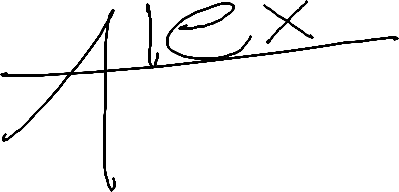
\includegraphics[height=7mm]{logo/FIRMA_Alex_Aravena_transparente.png}\\[-1pt]
        \rule{3.4cm}{0.4pt}
      \end{tabular}%
    }\\[-1pt]
    {\intermedium\fontsize{9pt}{11pt}\selectfont\color{lafroxTinta}%
      \LFXfoliotexto}
  \end{tabular}%
  \endgroup
}
